% radarnet_dsp_mac_engine.tex — Fig. 3: one output lane of the W×W PE array and its
% requantization pipeline (W = 8 shown). All W lanes are identical and run in parallel.
% Build: pdflatex radarnet_dsp_mac_engine.tex  →  radarnet_dsp_mac_engine.pdf
\documentclass[border=3pt]{standalone}
\usepackage{tikz}
\usetikzlibrary{positioning,arrows.meta,calc,backgrounds}
\begin{document}
\sffamily\footnotesize
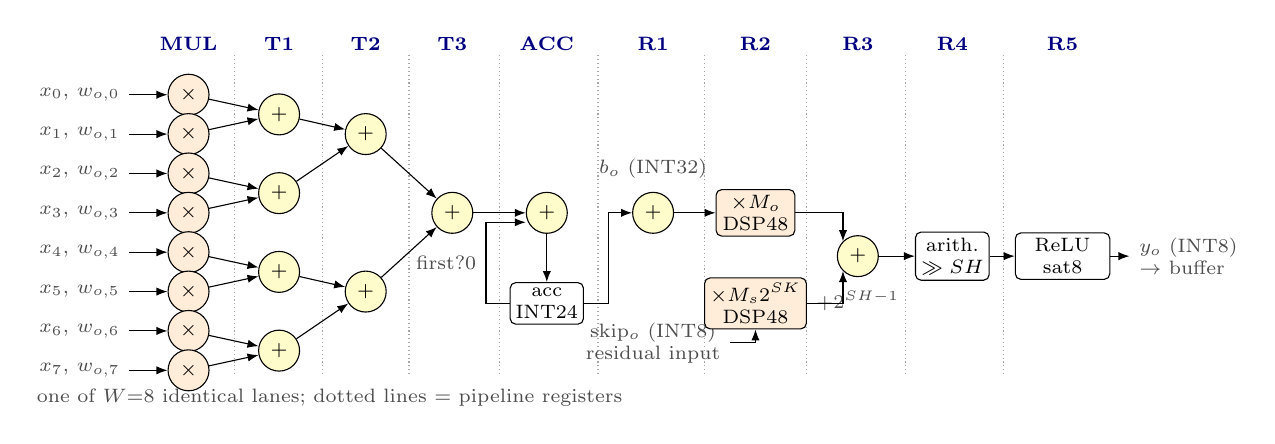
\begin{tikzpicture}[
  op/.style={draw, circle, minimum size=5.2mm, inner sep=0pt, fill=white, font=\scriptsize},
  mul/.style={op, fill=orange!15},
  add/.style={op, fill=yellow!20},
  blk/.style={draw, rounded corners=2pt, align=center, inner sep=2pt, fill=white, font=\scriptsize},
  dsp/.style={blk, fill=orange!15},
  wire/.style={-{Latex[length=1.4mm]}},
  lbl/.style={font=\scriptsize, text=black!70},
  stage/.style={font=\scriptsize\bfseries, text=blue!50!black}]

% ---------------- inputs and multipliers ----------------
\foreach \i in {0,...,7} {
  \pgfmathsetmacro{\y}{3.5-0.5*\i}
  \node[lbl, anchor=east] (x\i) at (0,\y) {$x_{\i},\,w_{o,\i}$};
  \node[mul] (m\i) at (0.75,\y) {$\times$};
  \draw[wire] (x\i) -- (m\i);
}
% ---------------- adder tree (3 registered levels for W = 8) ----------------
\foreach \j in {0,...,3} {
  \pgfmathtruncatemacro{\a}{2*\j}\pgfmathtruncatemacro{\b}{2*\j+1}
  \pgfmathsetmacro{\y}{3.25-1.0*\j}
  \node[add] (a1\j) at (1.9,\y) {$+$};
  \draw[wire] (m\a) -- (a1\j); \draw[wire] (m\b) -- (a1\j);
}
\foreach \j in {0,1} {
  \pgfmathtruncatemacro{\a}{2*\j}\pgfmathtruncatemacro{\b}{2*\j+1}
  \pgfmathsetmacro{\y}{3.0-2.0*\j}
  \node[add] (a2\j) at (3.0,\y) {$+$};
  \draw[wire] (a1\a) -- (a2\j); \draw[wire] (a1\b) -- (a2\j);
}
\node[add] (a3) at (4.1,2.0) {$+$};
\draw[wire] (a20) -- (a3); \draw[wire] (a21) -- (a3);

% ---------------- accumulator ----------------
\node[add] (acc) at (5.3,2.0) {$+$};
\node[blk, minimum width=9mm] (accr) at (5.3,0.85) {acc\\ INT24};
\draw[wire] (a3) -- (acc);
\draw[wire] (acc.south) -- (accr.north);
\draw[wire] (accr.west) -- ++(-0.3,0) |- node[lbl, pos=0.25, left] {first?0} ([yshift=-1.2mm]acc.west);

% ---------------- requantization pipeline ----------------
\node[add] (r1) at (6.65,2.0) {$+$};
\node[lbl, above=0.5mm of r1] {$b_o$ (INT32)};
\draw[wire] (accr.east) -| ([xshift=-3mm]r1.west) -- (r1.west);
\node[dsp, minimum width=10mm] (r2) at (7.95,2.0) {$\times M_o$\\ DSP48};
\draw[wire] (r1) -- (r2);
\node[lbl, align=center] (skin) at (6.65,0.35) {skip$_{o}$ (INT8)\\ residual input};
\node[dsp, minimum width=10mm] (r2s) at (7.95,0.85) {$\times M_s 2^{SK}$\\ DSP48};
\draw[wire] (skin.east) -| (r2s.south);
\node[add] (r3) at (9.25,1.45) {$+$};
\node[lbl, below=0.5mm of r3] {$+2^{SH-1}$};
\draw[wire] (r2.east) -| (r3.north west);
\draw[wire] (r2s.east) -| (r3.south west);
\node[blk, minimum width=9mm] (r4) at (10.45,1.45) {arith.\\ $\gg SH$};
\node[blk, minimum width=12mm] (r5) at (11.85,1.45) {ReLU\\ sat8};
\draw[wire] (r3) -- (r4);
\draw[wire] (r4) -- (r5);
\node[lbl, anchor=west, align=left] (y) at (12.7,1.45) {$y_o$ (INT8)\\ $\rightarrow$ buffer};
\draw[wire] (r5) -- (y);

% ---------------- pipeline stage markers ----------------
\foreach \x/\t in {0.75/{MUL}, 1.9/{T1}, 3.0/{T2}, 4.1/{T3}, 5.3/{ACC}, 6.65/{R1}, 7.95/{R2},
                   9.25/{R3}, 10.45/{R4}, 11.85/{R5}}
  \node[stage] at (\x,4.15) {\t};
\begin{scope}[on background layer]
  \foreach \x in {1.33,2.45,3.55,4.7,5.95,7.3,8.6,9.85,11.1}
    \draw[densely dotted, black!35] (\x,4.0) -- (\x,-0.05);
\end{scope}
\node[lbl, anchor=west] at (-1.3,-0.35) {one of $W{=}8$ identical lanes; dotted lines = pipeline registers};
\end{tikzpicture}
\end{document}
